\subsection{Cube-line picking and related generalizations}
\label{sec:cube_line}

These results have also been extended into 3D, with the probability
density function of distances between two (uniformly) randomly chosen
points in the unit cube is given in
\cite{mathai99:_distan,weisstein:_cube_line_picking}, by a yet more
complicated, but again easily evaluated formula. Likewise the formula
have been calculated for a box (with sides $a,b$ and
$c$)~\cite{philip:_probab_distr_distan_between_two} and 4- and
5-Cubes~\cite{philip:_probab_distr_distan_between_two_4d}. Other
results are also known, for instance the distribution when the points
are chosen on the sides of the square (but lines are drawn across it)
or faces of a cube!\cite{mathai99:_distan}, and the distribution of
distances between points chosen in two different
rectangles~\cite{b.ghosh51:_random_rect}.

Figures ...
 
\begin{figure}[tbp]
  \begin{center}
    \subfloat[\label{fig:cube_eg}Example.]
         {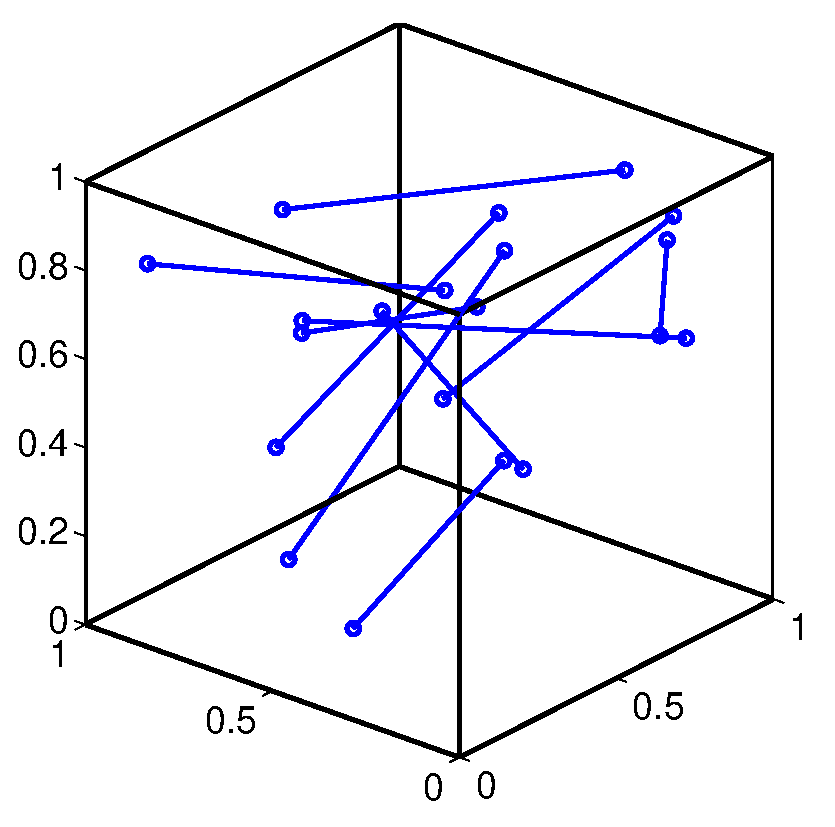
\includegraphics[width=0.47\columnwidth]{../Matlab/Plots/LinePicking_eg_cube.eps}}
    \hspace{3mm}
    \subfloat[\label{fig:cube_pdf}The PDF for $a=1$, $b=2.5$, showing the two regions.]
        {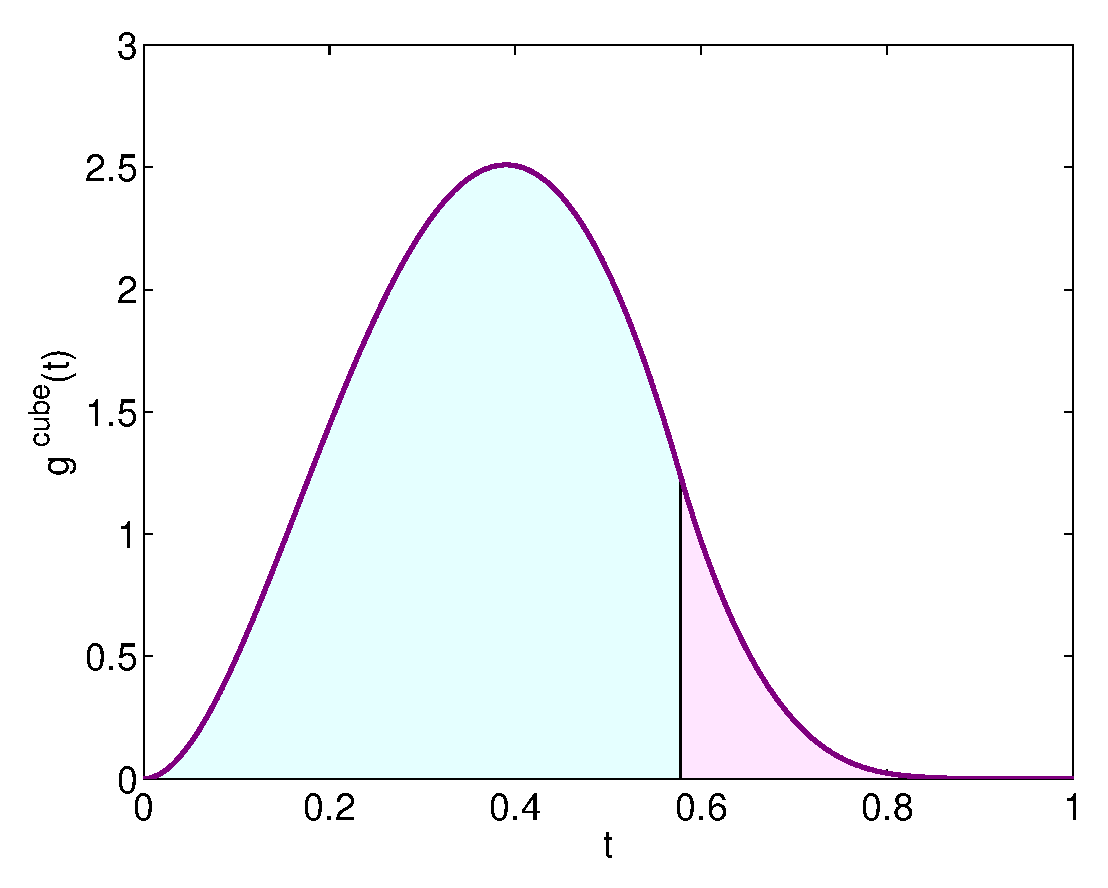
\includegraphics[width=0.47\columnwidth]{../Matlab/Plots/LinePicking_plot_cube_regions.eps}}
    \caption{Line-picking problem on the cube.}
  \end{center} 
\vspace{-4mm}
\end{figure}

\subsubsection{PDF}

Maybe too complicated to write here???

Box and 4- and 54-cubes definitely are


\subsubsection{CDF}


\subsubsection{Moments}

The mean for the cube, known as the {\em Robbins constant}, is given
in \cite{robbins78:_constant,weisstein:_cube_line_picking} as
\begin{equation}
   \label{eq:cube_mean}
 \mu^{\rm cube} = \frac{1}{105} \left[ 
                             4 + 17 \sqrt{2}- 6 \sqrt{3}  +
                             21 \ln(1+\sqrt{2}) + 
                             42 \ln(2+\sqrt{3}) - 7 \pi
                      \right]
	=	0.66170...
\end{equation}
but a closed form for the variance does not appear (only even moments
are reported). Even more complicated results appear for 4- and 5-Cubes in
5-Cubes~\cite{philip:_probab_distr_distan_between_two_4d}:
\begin{eqnarray}
 \mu^{\rm 4-cube} & = & 0.7776656535 ...    \label{eq:4-cube}, \\
 \mu^{\rm 4-cube} & = & 0.8785309152 ...     \label{eq:5-cube}.
\end{eqnarray}

The variance does not seem to be given in closed form ...

